\documentclass[a4paper,12pt]{article}
\usepackage[utf8]{ inputenc}
\usepackage[ngerman]{babel}
\usepackage[a4paper, left=2.5cm, right=2.5cm]{geometry}
\usepackage{graphicx}
\usepackage{subcaption}
\usepackage{fancyhdr}
\usepackage{pdfpages}
\usepackage{listings}
\usepackage{hyperref}
\usepackage[official]{eurosym}
\usepackage{float}

\pagestyle{fancy}
\lstset{
	language=Matlab,
	breaklines=true,
	morekeywords={matlab2tikz},
	keywordstyle=\color{blue},
	morekeywords=[2]{1}, keywordstyle=[2]{\color{black}},
	identifierstyle=\color{black},
	stringstyle=\color{mylilas},
	commentstyle=\color{mygreen},
	showstringspaces=false,
	mathescape=true
	emph=[1]{for,end,break},emphstyle=[1]\color{red},
}

\lhead{PV im Stromsystem – Strommarkt}
\chead{}
\rhead{Gruppe D}

\begin{document}
	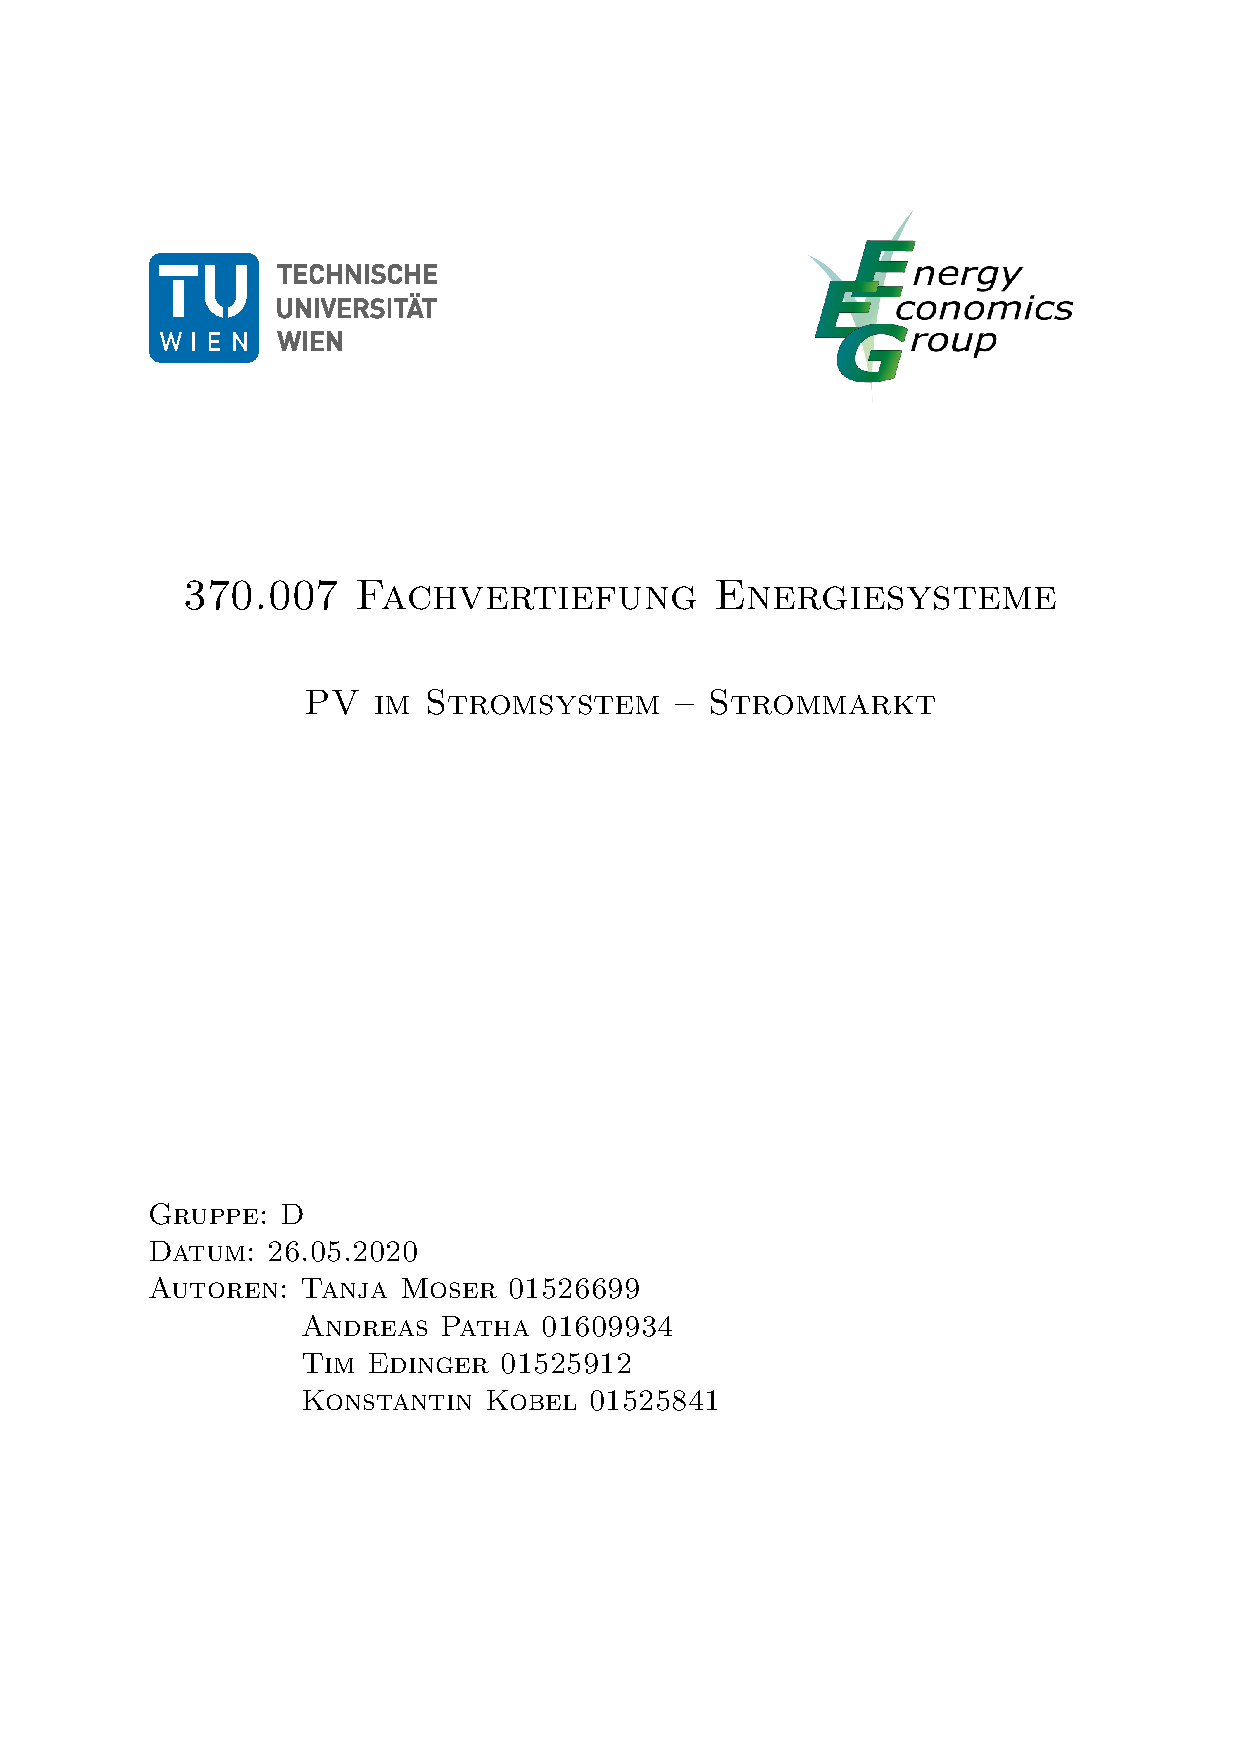
\includepdf{Protokoll_titlepage.pdf}

	\newpage
	\tableofcontents

	\newpage
	\section{Aufgabenstellung}
	\label{sec:Aufgabenstellung}
	In der vierten Übung sollen der Strommarkt und seine Entwicklung über die letzten Jahre, betrachtet werden. Besonders im Fokus stehen hierbei die Spotmarktpreise, die Stromerzeugung und die Netzlast, zu den unterschiedlichen Zeitpunkten.
	\subsection{Aufgabe 4.1}
	\label{sec:Aufgabenstellung41}
	In Aufgabe 4.1 sollen die Last und die Residuallast für das Marktgebiet Österreich/Deutschland, über ein Jahr, analysiert werden. Zusätzlich soll der Zusammenhang zwischen dem Spotmarktpreis und der Einspeisung von erneuerbaren Energien beleuchtet werden.\\ \par
	Folgende \textbf{Parameter} werden uns hierzu zur Verfügung gestellt:
	\begin{itemize}
		\item Die Datei $Load\_Production.mat$ beinhaltet die stündlichen Werte für die Netzlast (in $MW$) sowie die normierte PV-Erzeugung (in $MW/MW_{peak}$), über ein Jahr.
		\item In der Datei $Daten\_Preise\_Last\_2012.xlsx$ befinden sich stündliche Jahresdaten, aus dem Jahr 2012, zu der Netzlast, der Erzeugung durch PV- und Wind-Anlagen, sowie zu den Spotpreisen.
		\item Die Datei $Spotpreis.mat$ beinhaltet für die Jahre 2008 bis 2016 die mittleren stündlichen Spotmarktpreise, über das jeweilige Jahr, in $\mbox{\euro}/MWh$. Schaltjahre wurden bei $8760$ abgeschnitten.
	\end{itemize}
	\noindent Folgende \textbf{Aufgabenstellungen} sollen behandelt werden:
	\begin{itemize}
		\item[a)] Stellen Sie eine Dauerlinie der Last und der Residuallast ($Last - PV_{Produktion}$) für eine installierte Leistung von PV-Anlagen in der Höhe von 0 bis 200 GW dar. (in 50GW-Intervallen).\newline Was beobachten Sie?
		\item[b)] Betrachten Sie im Folgenden die tatsächlichen Daten der Erneuerbaren (Wind und PV) aus dem Jahr 2012. Stellen Sie die Last sowie Residuallast ($Last - PV_{Produktion} - Wind_{Produktion}$) als Leistungsdauerlinie dar.
		\item[c)] Erstellen Sie 3 Scatterplots (siehe Matlab-Funktion scatter) des Spotmarktpreises in Abhängigkeit von:
		\begin{itemize}
			\item Last
			\item Residuallast
			\item Einspeisung der Erneuerbaren
		\end{itemize}
		\item[d)] Wie interpretieren Sie die Scatterplots? Decken sich die Ergebnisse mit ihren Erwartungen?
	\end{itemize}
	\subsection{Aufgabe 4.2}
	\label{sec:Aufgabenstellung42}
	Das Ziel von Aufgabe 4.2 ist es die historische Entwicklung der Großhandelsstrompreise vom Jahr 2008 bis zum Jahre 2016 zu beschreiben.\\ \par
	\noindent	Die hierfür nötigen \textbf{Parameter} können dem Kapitel \hyperref[sec:Aufgabenstellung41]{Aufgabe 4.1} entnommen werden.\\ \par
	\noindent Die \textbf{Aufgaben} lauten:
	\begin{itemize}
		\item[a)] Erstellen Sie die Preisdauerlinie für die Jahre 2008 bis 2016.\newline Was beobachten Sie?
		\item[b)] Erstellen Sie eine Grafik der mittleren stündlichen Großhandelsstrompreise für alle 24h für die Jahre 2016 und 2008. Sprich für jede Stunde soll der Mittelwert aus 365 Tagen gebildet werden.
		\begin{itemize}
			\item Alternativ können Sie dies auch mit einem Boxplot darstellen.
			\item Was erkennen Sie daraus?
		\end{itemize}
	\end{itemize}
	\subsection{Aufgabe 4.3}
	\label{sec:Aufgabenstellung43}
	Aufgabe 4.3 befasst sich mit der Entwicklung des monetären Ertrags einer PV-Anlage, über die Jahre 2008 bis 2016.\\ \par
	\noindent Die dazu gegebenen \textbf{Parameter} sind folgende:
	\begin{itemize}
		\item Es wird von einer $1kWp$ PV-Anlage ausgegangen.
		\item Das Erzeugungsprofil der PV-Anlage ist in der Datei $Load\_PVProduction.mat$ enthalten.
	\end{itemize}
	Für den konkreten Fall aus Aufgabe 4.3 soll die Annahme getroffen werden, dass die komplette Erzeugung am Spotmarkt verkauft wird.\\ \par
	\noindent Speziell sollen folgende \textbf{Aufgaben} behandelt werden:
	\begin{itemize}
		\item[a)] Berechnen Sie den monetären Ertrag am Spotmarkt (Marktwert) einer $1kWp$-PV-Anlage für die Jahre 2008 bis 2016 (das PV-Erzeugungsprofil (in $MW/MW_{peak}$) finden Sie im File $Load\_PVProduction.mat$)
		\item[b)] Geben Sie die monetären Erträge (der $1kWp$-Anlage) der Tage 4 bis 34 und 180 bis 220 im Jahr 2008 und 2016 an.
		\item[c)] Wie interpretieren Sie die jährliche Entwicklung der Erträge? Was schließen Sie aus den Ergebnissen?
	\end{itemize}
	\newpage
	\section{Berechnungen}
	\label{sec:Berechnungen}
	\subsection{Last und Residuallast}
	Die \textbf{Last} bezeichnet in der elektrischen Energietechnik die gesamte, in einem Stromnetz nachgefragte, elektrische Leistung. \\ \par
	\noindent Die \textbf{Residuallast} bezeichnet in der elektrischen Energietechnik die in einem Stromnetz nachgefragte elektrische Leistung, abzüglich des Anteils fluktuierender Einspeisung von dargebotsabhängigen Erzeugern, wie Windkraft- oder PV-Anlagen. Die Residuallast ist demnach die Leistung, die von Regelkraftwerken gedeckt werden muss.\\ \par
	\noindent Die Berechnung der Residuallast erfolgt für den Fall aus \hyperref[sec:Aufgabenstellung41]{Aufgabe 4.1.a} wie folgt:
	\begin{equation}
	Residuallast = Last - PV_{Profil} * PV_{Leistung}
	\end{equation}
	\begin{itemize}
		\item \textbf{Last} ist die in der Datei $Load\_Production.mat$ zur Verfügung gestellte Netzlast.
		\item \textbf{PV-Profil} entspricht dem in der Datei $Load\_Production.mat$ enthaltenen Erzeugungsprofil einer PV-Anlage.
		\item \textbf{PV-Leistung} entspricht der installierten Leistung. Für den Fall aus \hyperref[sec:Aufgabenstellung41]{Aufgabe 4.1.a} soll die installierte Leistung von $0GW$ bis $200GW$, in $50GW$-Schritten variiert werden.
	\end{itemize}
	Im Falle von \hyperref[sec:Aufgabenstellung41]{Aufgabe 4.1.b} erfolgt die Berechnung der Residuallast über folgende Formel:
	\begin{equation}
	Residuallast = Last - PV_{Produktion} - Wind_{Produktion}
	\end{equation}
	\begin{itemize}
		\item \textbf{Last} ist die in der Datei $Daten\_Preise\_Last\_2012.xlsx$ zur Verfügung gestellte Netzlast, für das Jahr 2012.
		\item \textbf{PV-Produktion} entspricht der in der Datei $Daten\_Preise\_Last\_2012.xlsx$ enthaltenen PV-Einspeisung, für das Jahr 2012.
		\item \textbf{Wind-Produktion} entspricht der in der Datei $Daten\_Preise\_Last\_2012.xlsx$ enthaltenen Einspeisung aus Windkraft-Anlagen, für das Jahr 2012.
	\end{itemize}
	\newpage
	\subsection{Monetärer Ertrag einer 1kWp PV-Anlage}
	Der monetäre Ertrag einer PV-Anlage ergibt sich aus der Multiplikation der Kraftwerkleistung, den Profilwerten und dem jeweiligen Spotpreis. Durch Aufsummieren der einzelnen Werte eines Jahres, erhält man den gesamten monetären Ertrag des jeweiligen Jahres (in Euro).
	\begin{equation}
	Ertrag(a) = \sum\nolimits_{i=1}^n PV_{Leistung} * PV_{Profil,k} * Spotpreis_k(a)
	\end{equation}
	\begin{itemize}
		\item \textbf{Ertrag} entspricht dem gesamten monetären Ertrag eines Jahres, in Euro.
		\item \textbf{a} ist das entsprechende Jahr, für das der monetäre Ertrag errechnet werden soll. (in unserem Fall von 2008 bis 2016)
		\item \textbf{k} entspricht dem Intervall, in dem Daten vorhanden sind (in unserem Fall handelt es sich um stündliche Daten. Daraus folgt, dass \textbf{n} einem Wert von 8760 Stunden entspricht.).
		\item \textbf{PV-Leistung} ist die installierten Leistung der PV-Anlage. Für den Fall aus \hyperref[sec:Aufgabenstellung43]{Aufgabe 4.3} entspricht das $1kWp$.
		\item \textbf{PV-Profil} ist das Erzeugungsprofil der PV-Anlage.
		\item \textbf{Spotpreis} entspricht dem jeweiligen Spotpreis im Jahr $a$, zum Zeitpunkt $k$.
	\end{itemize}
	\newpage
	\section{Ergebnisse}
	\label{sec:Ergebnisse}
	\subsection{Aufgabe 4.1 - Last und Residuallast}
	\subsubsection{Aufgabe 4.1.a - Dauerlinie der Last und der Residuallast}
	\begin{figure}[H]
		\centering
		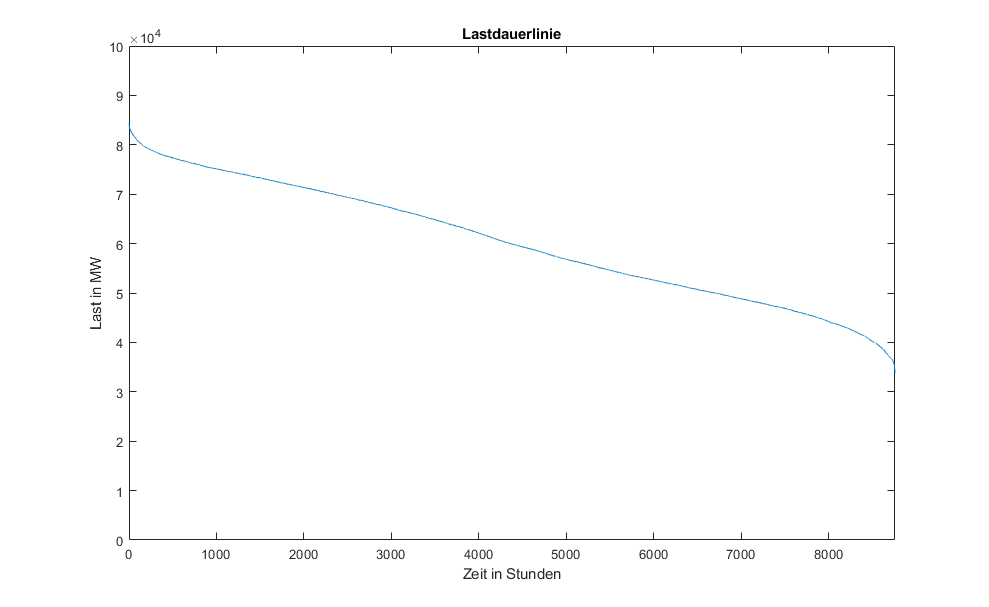
\includegraphics[width=12cm]{img/results/Lastdauerlinie}
		\caption{TODO!}
	\end{figure}
	\begin{figure}[H]
		\centering
		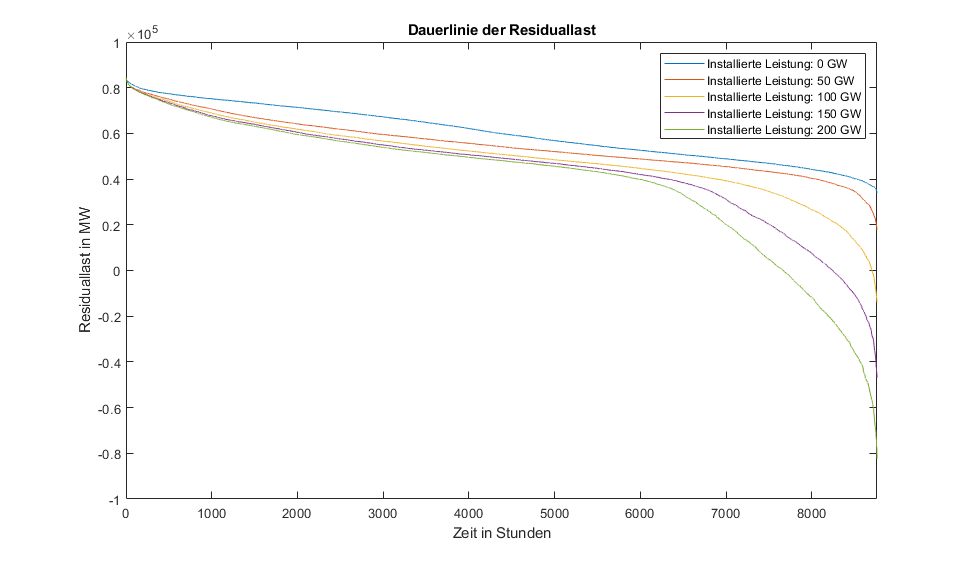
\includegraphics[width=12cm]{img/results/DauerlinieResiduallast}
		\caption{TODO!}
	\end{figure}
	\subsubsection{Aufgabe 4.1.b - Dauerlinie der Last und der Residuallast für das Jahr 2012}
	\begin{figure}[H]
		\centering
		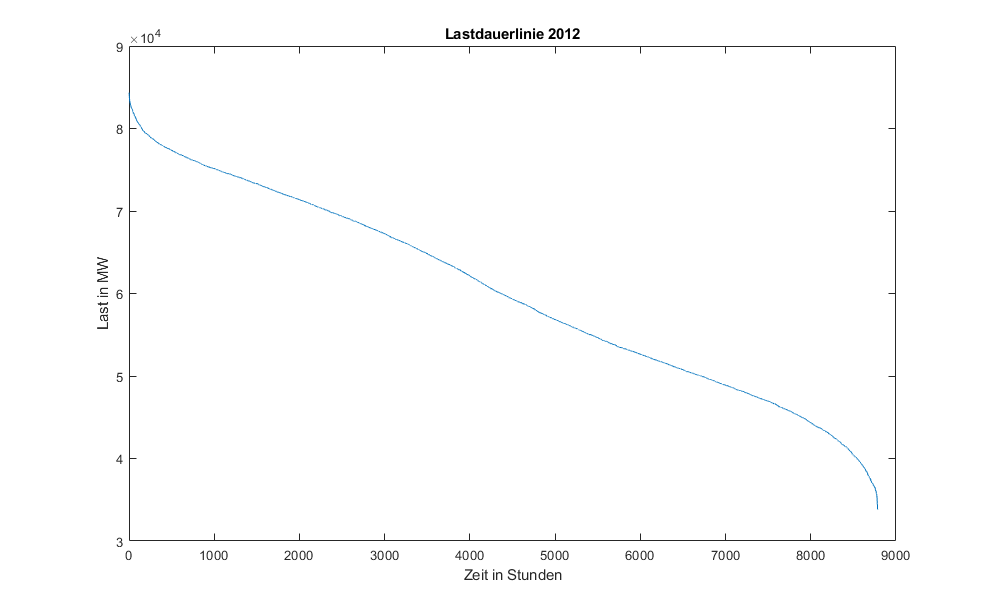
\includegraphics[width=12cm]{img/results/Lastdauerlinie2012}
		\caption{TODO!}
	\end{figure}
	\begin{figure}[H]
		\centering
		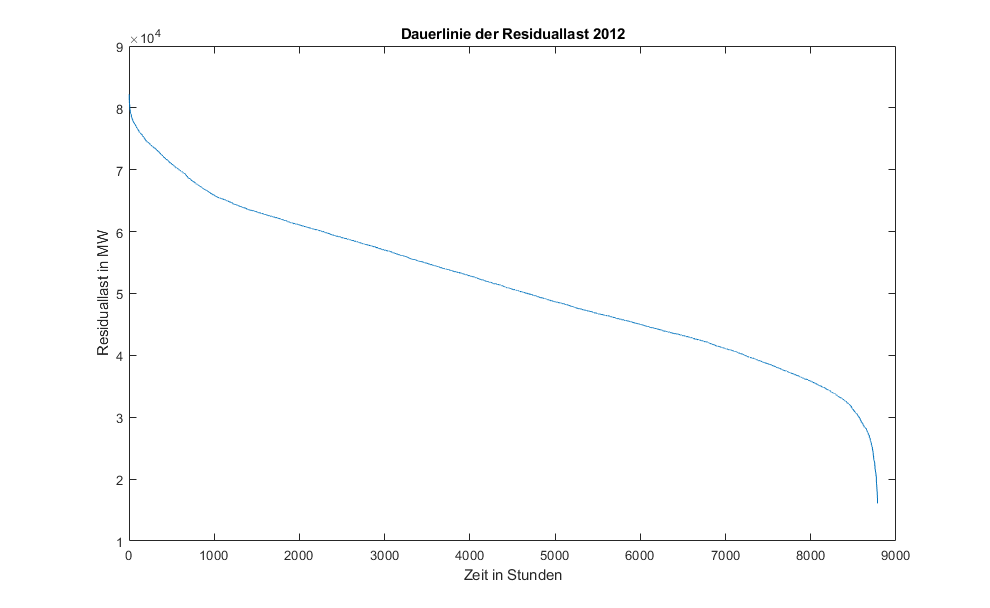
\includegraphics[width=12cm]{img/results/DauerlinieResiduallast2012}
		\caption{TODO!}
	\end{figure}
	\subsubsection{Aufgabe 4.1.c - Abhängigkeiten des Spotmarktpreises}
	\begin{figure}[H]
		\centering
		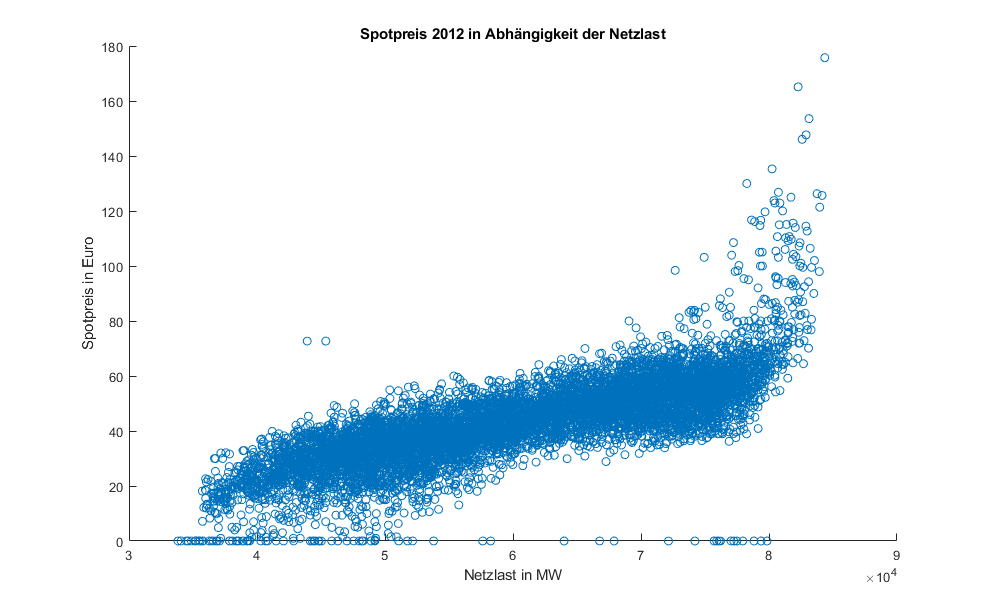
\includegraphics[width=12cm]{img/results/ScatterNetzlast}
		\caption{TODO!}
	\end{figure}
	\begin{figure}[H]
		\centering
		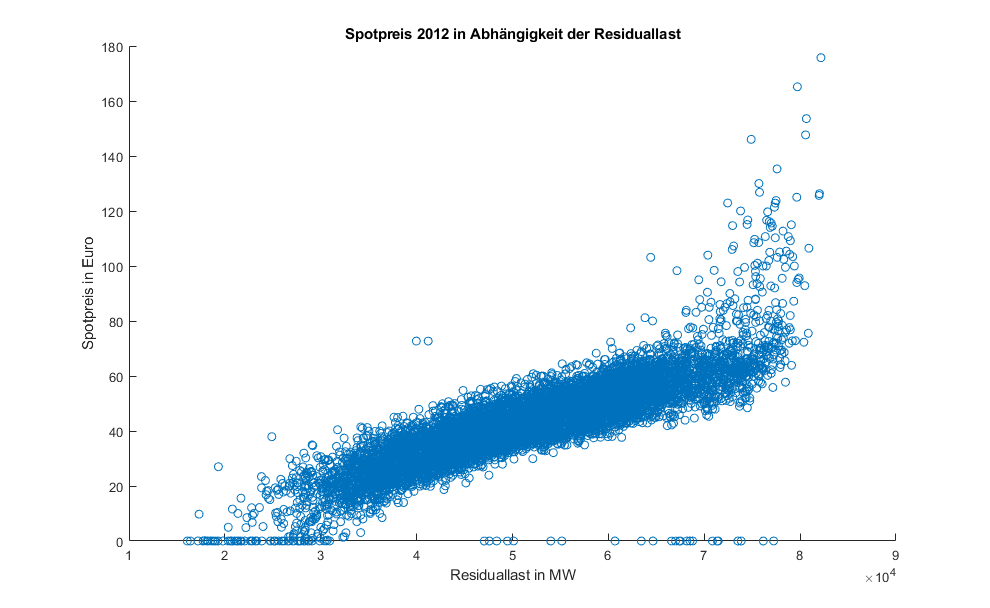
\includegraphics[width=12cm]{img/results/ScatterResiduallast}
		\caption{TODO!}
	\end{figure}
	\begin{figure}[H]
		\centering
		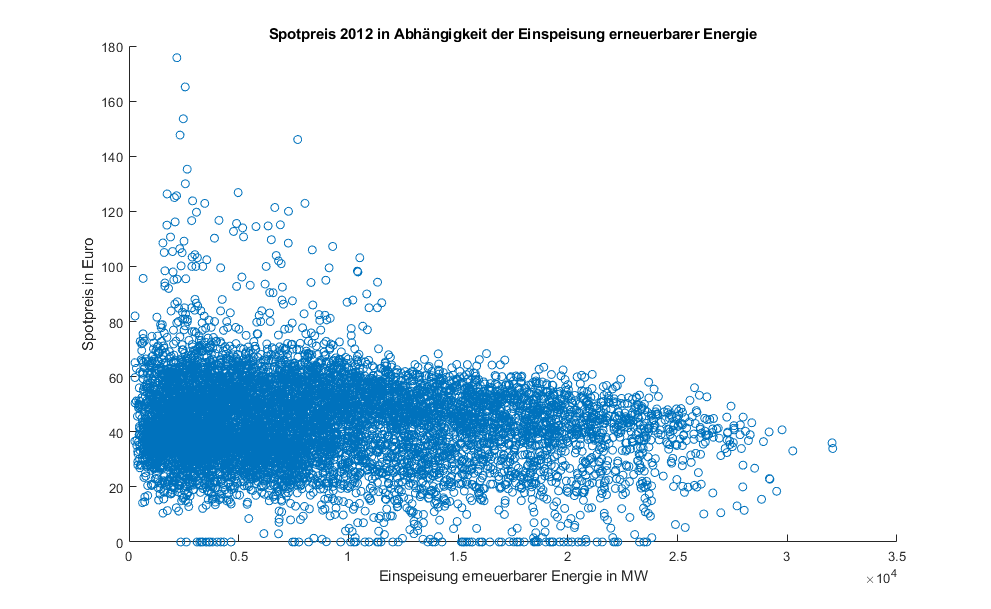
\includegraphics[width=12cm]{img/results/ScatterEinspeisung}
		\caption{TODO!}
	\end{figure}
	\subsubsection{Aufgabe 4.1.d - Interpretation der Scatter-Plots}
	\begin{enumerate}
		\item Der Scatter-Plot in Abbildung 5 stellt den Spotmarktpreis, in Abhängigkeit der Netzlast dar.\newline
		
		
		\item In Abbildung 6 ist der Spotmarktpreis, in Abhängigkeit der Residuallast dargestellt.\newline
		
		\item Abbildung 7 stellt den Spotmarktpreis in Abhängigkeit der Einspeisung erneuerbarer Energie dar.\newline
	\end{enumerate}
	Zusammenfassen kann man sagen, dass sich die Ergebnisse mit unseren Erwartungen decken. Es ist ein allgemeiner Zusammenhang zwischen der Nachfrage nach Energie und dem Spotmarktpreis ersichtlich.\newline Sobald eine hohe Nachfrage besteht, die fluktuierender Einspeisung von dargebotsabhängigen Erzeugern jedoch gering ist (Aufgrund der aktuellen Jahreszeit, des Wetters, etc.), steigt der Spotmarktpreis.\newline
	Besteht eine geringe Nachfrage während die Einspeisung durch erneuerbare Energien jedoch hoch ist (z.B. zur Mittagszeit im Sommer), sinkt der Spotmarktpreis.
	\newpage
	\listoffigures
\end{document}